
\documentclass[12pt,a4paper]{report}
\usepackage{sectsty}
\pagestyle{empty}
\pagestyle{plain}
\chaptertitlefont{\large}
\usepackage[utf8]{inputenc}
\usepackage[brazil]{babel}
%\usepackage{graphics}
\usepackage{lineno,hyperref}
\usepackage{xcolor}
\usepackage{amsmath}
\usepackage{numberedblock}
\usepackage{float}
% \usepackage{booktabs}
\usepackage{graphicx}
 
\usepackage{hyperref}
\hypersetup{
    colorlinks=true,
    linkcolor=blue,
    filecolor=magenta,      
    urlcolor=cyan,
}
\usepackage{booktabs}
\usepackage{longtable}
\usepackage{upgreek}
\usepackage{algorithm2e}
\usepackage{graphicx}
\usepackage{listings}

\usepackage{algorithm}
\usepackage[noend]{algpseudocode}

\usepackage{minted}



\usepackage{graphicx,url}
\usepackage[top=2cm, bottom=2cm, left=2.5cm, right=2.5cm]{geometry}
\usepackage{enumitem}
\hyphenpenalty=5000 
\tolerance=1000


\begin{document}
	\begin{center}
		
		{\LARGE  Universidade Federal de Santa Catarina – UFSC}
	    \large Programa de Pós-Graduação em Engenharia Elétrica – CTC
	
		\large EEL510265 – Programação de Sistemas Embarcados – 2019/2
		\end{center}
		\begin{center}
		\large {Cezar Antônio Rigo – 201902714}
			\end{center}

    	\begin{center}
		{\Large \textbf{\\ Relatório Final: }}
		\vspace{5pt}
		{\Large \textbf{\\ Máquina de Vendas Escalonada}}
    	\end{center}
	
\vspace{20pt}

Este relatório apresenta o processo de desenvolvimento da solução completa para o trabalho final da disciplina, programadado em C++.  

\large
\vspace{20pt}
 \textbf {1. Diagrama das classes implementadas}
\vspace{10pt}
\normalsize

A Figura \ref{fig:diag_cla_atual} apresenta o diagrama das classes implementadas a fim de cumprir as especificações funcionais e requisitos do trabalho final. As classes BancoDados e Machine (em verde) são \textbf{friends} e isso foi feito para que a classe BancoDados possa ter acesso a interface, objeto de Machine, especialmente para mostrar o relatório final de vendas. 


Para atender ao requisito de portabilidade do código C++ para diferentes interfaces, foi criada uma classe Interface pai com funções virtuais e duas classes derivadas, a InterfaceAtl para o sistema embarcado alvo e a InterfacePC para execução no microcomputador. Dessa forma faz-se uso do \textbf{polimorfismo} e da condicional \#ifdef para definir qual classe instanciar, de acordo com a plataforma alvo.



\begin{figure}[H]
    \begin{center}
        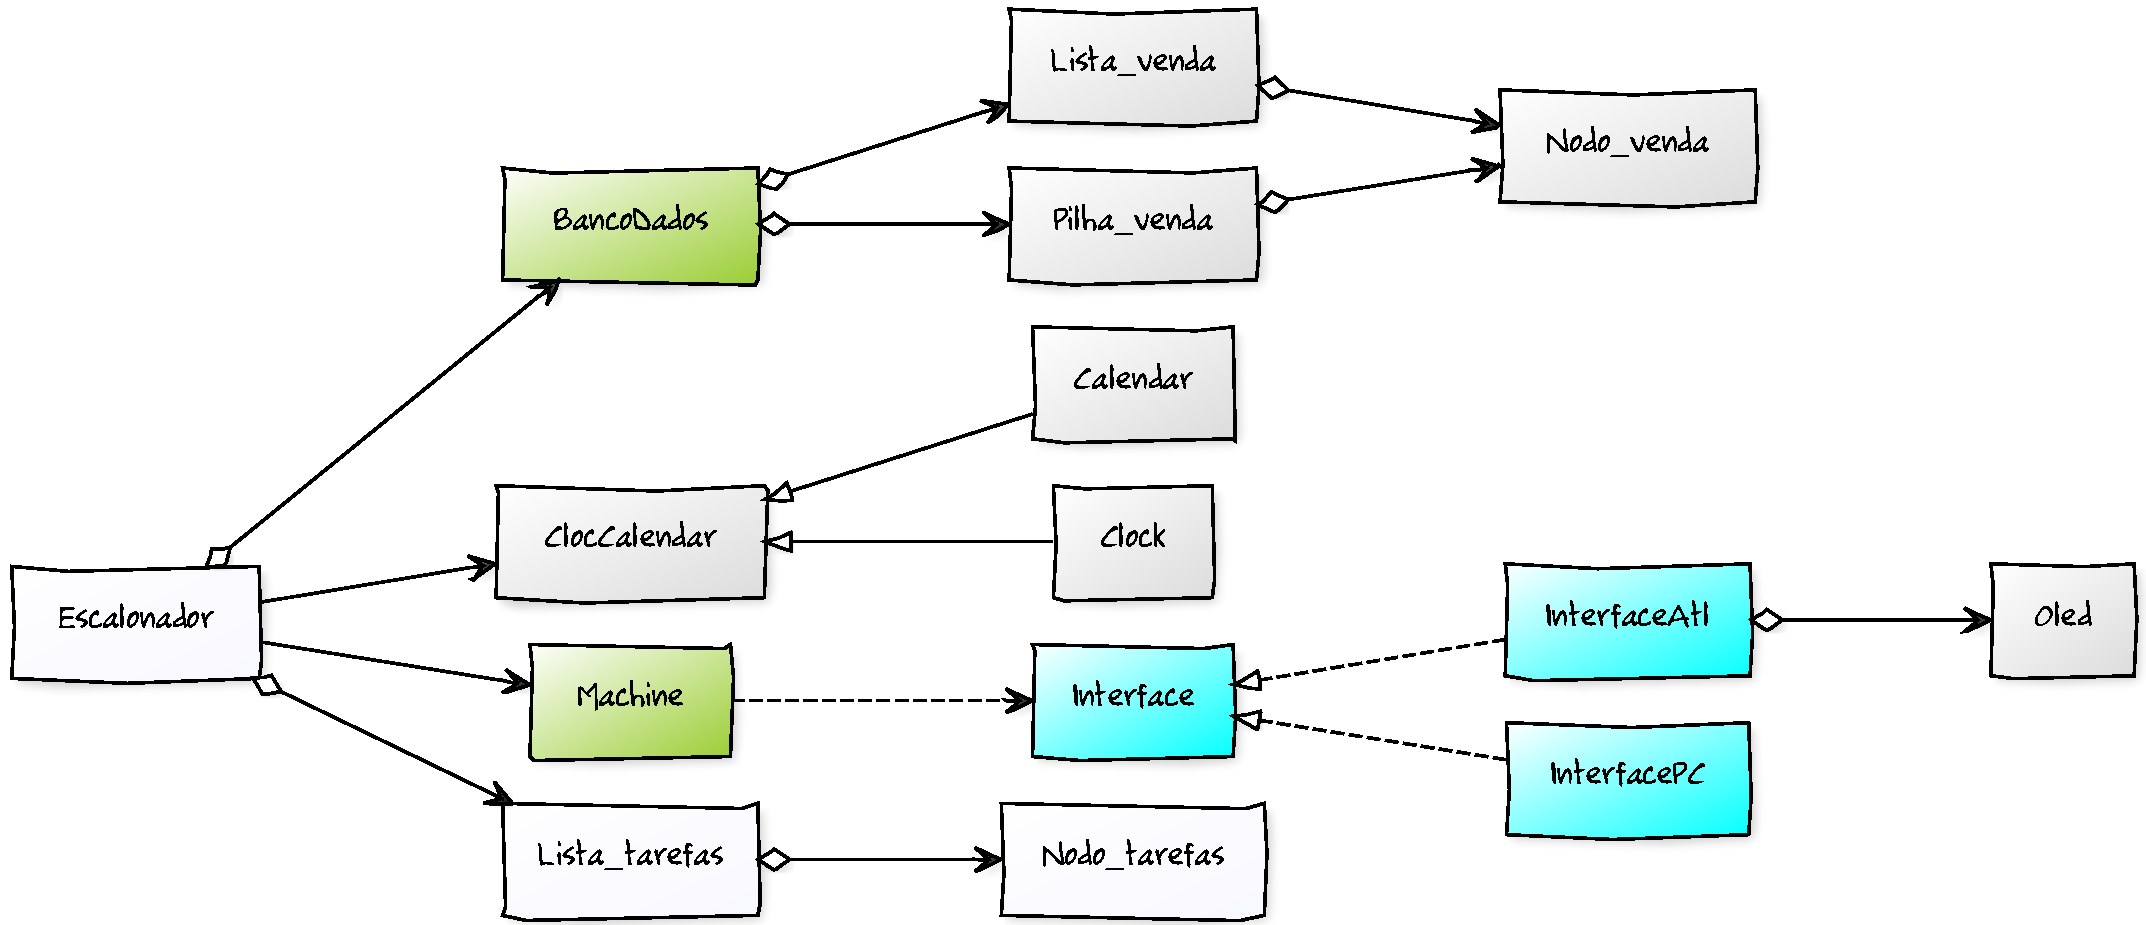
\includegraphics[width=1\textwidth]{diag_cla_atual.pdf}
        \caption{\small{Diagrama das classes implementadas.}}
        \label{fig:diag_cla_atual}
    \end{center}
\end{figure}

Nas próximas seções serão detalhados o funcionamento da máquina de vendas, do banco de dados, do escalonador e do ClockCalendar.


\large
\vspace{20pt}
 \textbf {2. A máquina de vendas}
\vspace{10pt}
\normalsize


 A Figura \ref{fig:diag_cla_mach} traz o diagrama expandido das classes relacionadas à venda de refrigerantes. Essa classe é responsável por gerenciar todo processo de venda, bem como permitir acesso às interfaces. 

\begin{figure}[H]
    \begin{center}
        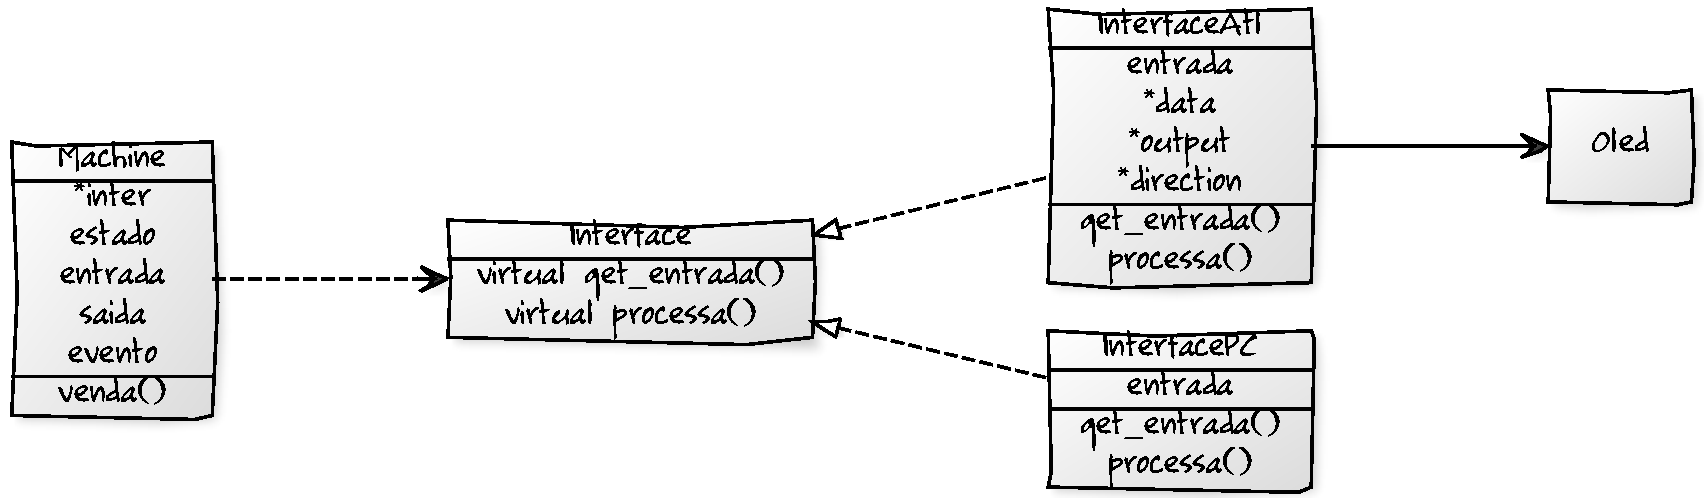
\includegraphics[width=0.95\textwidth]{diag_cla_mach.pdf}
        \caption{\small{Diagrama expandido das classes relacionadas à venda de refrigerantes.}}
        \label{fig:diag_cla_mach}
    \end{center}
\end{figure}

Esse acesso é dado através do ponteiro *inter, do tipo Interface, possibilitando executar as funções get\_entrada(), que obtém input do usuário, e processa(), que mostra as saídas da máquina. O polimorfismo se dá através da criação de uma classe pai que possui as mesmas funções, porém declaradas como virtuais puras. O ponteiro inter aponta para InterfacePC ou interfaceATL conforme definição do usuário. O código a seguir mostra esta sintaxe:

\begin{minted}
[
fontsize=\small,
linenos
]{cpp}
#ifdef PC
    inter = new InterfacePc;
#endif

#ifdef ATL
    inter = new InterfaceAtl;
#endif

entrada = inter->get_entrada(); //chama objeto interface para 
obter entrada
\end{minted}

Para que o controlador da máquina de venda de refrigerantes funcionasse de acordo com as especificações de projeto, foi solucionada a Tabela \ref{tab:my-table} que abrange todas as  possibilidades de entrada e correspondentes mudanças estados. 

\begin{table}[h]
\caption{Solução da tabela de estados}
\label{tab:my-table}
\resizebox{\textwidth}{!}{%
\begin{tabular}{@{}llllllll@{}}
\toprule
\textbf{Estado Atual} & \textbf{Nada} & \textbf{M025} & \textbf{M050} & \textbf{M100}    & \textbf{DEV}     & \textbf{MEET} & \textbf{ETIRPS} \\ \midrule
\textbf{S000}         & S000          & S025          & S050          & S100             & S000             & S000          & S000            \\
\textbf{S025}         & S025          & S050          & S075          & S125             & S000, D025       & S025          & S025            \\
\textbf{S050}         & S050          & S075          & S100          & S150             & S000, D050       & S050          & S050            \\
\textbf{S075}         & S075          & S100          & S125          & S150, D025       & S000, D025, D050 & S075          & S075            \\
\textbf{S100}         & S100          & S125          & S150          & S150, D050       & S000, D100       & S100          & S100            \\
\textbf{S125}         & S125          & S150          & S150, D025    & S150, D025, D050 & S000, D100, D025 & S125          & S125            \\
\textbf{S150}         & S150          & S150, D025    & S150, D050    & S150, D100       & S000, D100, D050 & MEET          & ETIRPS          \\ \bottomrule
\end{tabular}%
}
\end{table}

A implementação das máquinas de estado em C++ se deu dentro da classe Machine, na função venda() – vide Figura \ref{fig:diag_cla_mach}. A classe Machine possui as variáveis estado, entrada, saida e evento para armazenar o estado atual da maquina bem como a entrada e assim determinar a saída. Após obtenção do valor da entrada, através da chamada da classe Interface apropriada, a transição de estados é determinada através de switch-case, conforme apresentado no fragmento de código abaixo:

\begin{minted}
[
fontsize=\small,
linenos
]{cpp}
    switch (estado)
    {
    case 0:
        if (entrada == "m025")
            estado = 25;

        else if (entrada == "m050")
            estado = 50;

        else if (entrada == "m100")
            estado = 100;

        entrada = "nada";
        break;
    ...
    }
\end{minted}


A vantagem desta implementação é que na ocorrência de uma interrupção não há chance de perda do estado atual da máquina, tampouco da entrada mais recente, já que estes valores estão armazenados no objeto Machine, através de variáveis – vide Figura \ref{fig:diag_cla_mach}. Assim que um valor de entrada for obtido a máquina passa pelo switch-case, se necessário a Interface é chamada novamente para processar uma saída, e a execução da função venda() é terminada, permitindo retorno ao escalonador.


\large
\vspace{20pt}
 \textbf {3. O banco de dados}
\vspace{10pt}
\normalsize


 A classe BancoDados é responsável por  gerenciar uma pilha para armazenamento temporário dos dados de venda (classe Pilha\_venda) e uma lista para armazenamento definitivo (classe Lista\_venda). O diagrama expandido das classes relacionadas é apresentado na Figura \ref{fig:diag_cla_bd}.
 
 \begin{figure}[H]
    \begin{center}
        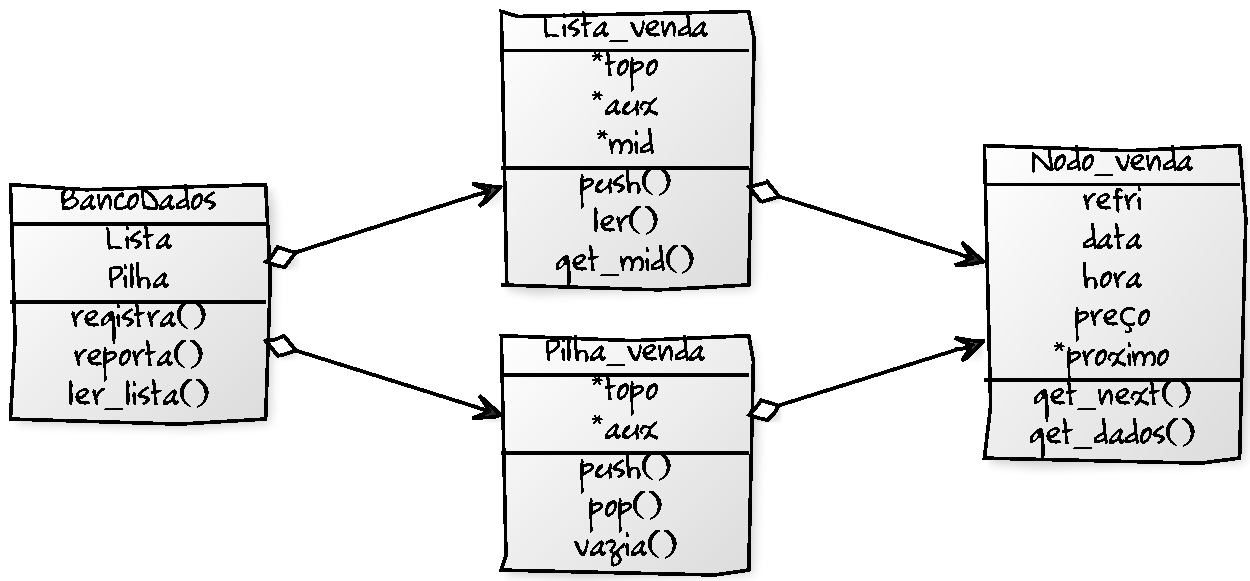
\includegraphics[width=0.75\textwidth]{diag_cla_bd.pdf}
        \caption{\small{Diagrama expandido das classes relacionadas ao gerenciamento dos dados de venda.}}
        \label{fig:diag_cla_bd}
    \end{center}
\end{figure}

O nodo contém todos os dados relacionados a uma venda, bem como o endereço de memória onde se encontra o próximo nodo, e é uma classe comum a ambas estruturas de dados (pilha e lista). A lista gerencia seus nodos com o auxilio de ponteiros do tipo nodo, o ponteiro "topo", por exemplo, sempre aponta para o último nodo na sequência, sendo que nodos nunca são excluídos. A classe pilha gerencia seus nodos de forma similar, porém ao fazer a leitura de um nodo - pop() - este é excluído. A criação e exclusão de nodos é feita com alocação dinâmica de memória, através dos comandos "new" e "delete". Sempre que uma venda for realizada o fragmento de código abaixo é executado, a fim de salvar as informações da venda:

\begin{minted}
[
fontsize=\small,
linenos
]{cpp}
#include <exception>
using std::bad_alloc;

void Pilha::push(string refri, int preco)
{
    /*  Funçao para inserir valores em um novo nodo da Pilha. 
    Argumentos:
    refri: O refrigerante vendido.
    g_data: A data da venda.
    g_hora: A hora da venda.
    precp: O preco do refrigerante.
   */
    try
    {   //aux recebe o endereco do novo nodo criado com o comando new.
        aux = new Nodo(refri, g_data, g_hora, preco, topo);
        topo = aux; //topo passa a apontar para o novo nodo.
    }
    catch (bad_alloc E)
    {
        cout << "Faltou Memoria...\n" << endl;
    }
}
\end{minted}

Como pode ser visto, foi usado também o \textbf{tratamento de exceções} para monitorar se faltou memória para executar o comando new.

Quando há alocação dinâmica de memória em uma classe com o uso de ponteiros, como é o caso, deve-se fazer um destrutor para liberar essa memória antes que a instância seja destruída. Dessa forma, tanto a classe Pilha quanto Lista possuem destrutores. Abaixo o código destrutor da classe Pilha: 

\begin{minted}
[
fontsize=\small,
linenos
]{cpp}
Pilha::~Pilha() //destroi a Pilha.
{
    while (topo) //enquanto houver um nodo.
    {
        aux = topo->get_next(); //salva o endereço para o proximo nodo.
        delete topo;            //deleta o nodo atual.
        topo = aux;             //atual = proximo.
    }

    //zera todos os ponteiros.
    topo = 0;
    aux = 0;
}                                       
}
\end{minted}

A classe BancoDados, por sua vez, tem uma função para registrar dados que chama a função push da pilha, criando um novo nodo. Também possui uma função reporta() que lê toda pilha atual, efetivamente esvaziando-a, processa os dados lidos para determinar o período de maior venda, o refrigerante mais vendido e o valor total de vendas e salva as informações (que estavam na pilha) na lista - armazenamento permanente. Este algoritmo é apresentado no pseudocódigo abaixo:

\begin{minted}
[
fontsize=\small,
linenos
]{cpp}
 Enquanto a pilha nao estiver vazia
    
        Retira dados da Pilha 
        
        Analisa qual refrigerante foi vendido e incrementa seu contador
       
        Verifica em qual periodo ocorreu a venda e incrementa seu contador
        
        Salva dados na Lista.
       
Analisa os contadores de periodo de vendas e define o maior
    
Analisa os contadores de refrigerante mais vendido e define o maior

Chama a interface para reportar
\end{minted}


Também chama uma função da interface para mostrar as informações de venda. Há, ainda, uma função para ler toda a lista, e assim mostrar todo o histórico de vendas.


\large
\vspace{20pt}
 \textbf {4. O Clock e Calendário}
\vspace{10pt}
\normalsize

A função advance() da classe ClockCalendar é executada pelo escalonador a cada segundo, para atualizar a hora. Essa classe \textbf{herda} das classes Clock e Calendar, como apresentado na Figura \ref{fig:diag_cla_clock}. 


\begin{figure}[H]
    \begin{center}
        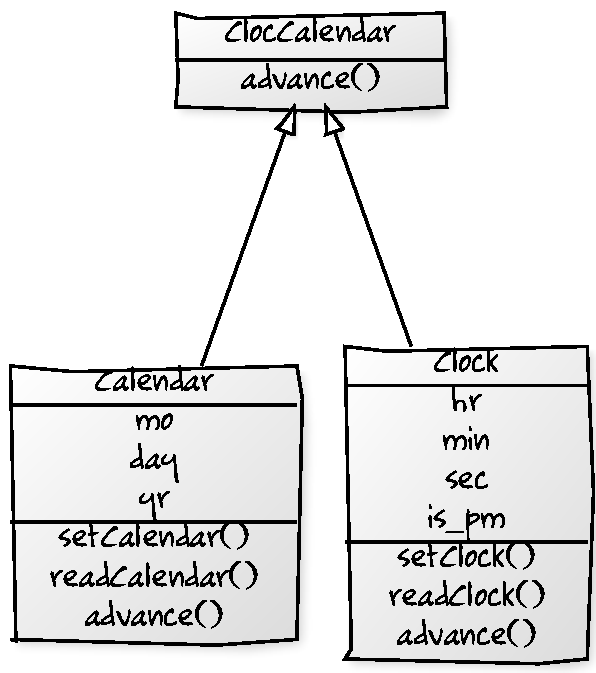
\includegraphics[width=0.34\textwidth]{diag_cla_clock.pdf}
        \caption{\small{Diagrama expandido das classes hora e data.}}
        \label{fig:diag_cla_clock}
    \end{center}
\end{figure}

As informações de data e hora são obtidas chamando readCalendar() e readClock(), também chamadas a cada segundo, e posteriormente salvas em variáveis globais para que as outras classes possam acessar. Há, ainda, uma \textbf{sobrecarga de operadores} para permitir avançar o calendário apenas digitando ++ObjetoClockCalendar;. Abaixo o fragmento de código usado para criar essa sobrecarga:
  
\begin{minted}
[
fontsize=\small,
linenos
]{cpp}

void operator++(ClockCalendar &t)
{
    t.advance();
}
\end{minted}


\large
\vspace{20pt}
 \textbf {5. O escalonador}
\vspace{10pt}
\normalsize


Para atender aos requisitos de escalonamento do projeto, as classes da Figura \ref{fig:diag_cla_esc} foram implementadas. O nodos, da classe Nodo\_tarefas possuem as informações de cada tarefa, como: atraso, período, status (apta ou bloqueada) e ponteiro para função associada. A cada 1 milissegundo a função executa() da classe Escalonador (Figura \ref{fig:diag_cla_esc}) é chamada. Essa função incrementa um contador de tempo e chama a função decide(), da Lista\_tarefas. Esta função tem acesso a todos os nodos, e baseado nessas informações e na passagem de tempo um algoritmo decide qual tarefa deve ser chamada e chama-a. O código desse algoritmo está anexado no APÊNDICE 1.


\begin{figure}[H]
    \begin{center}
        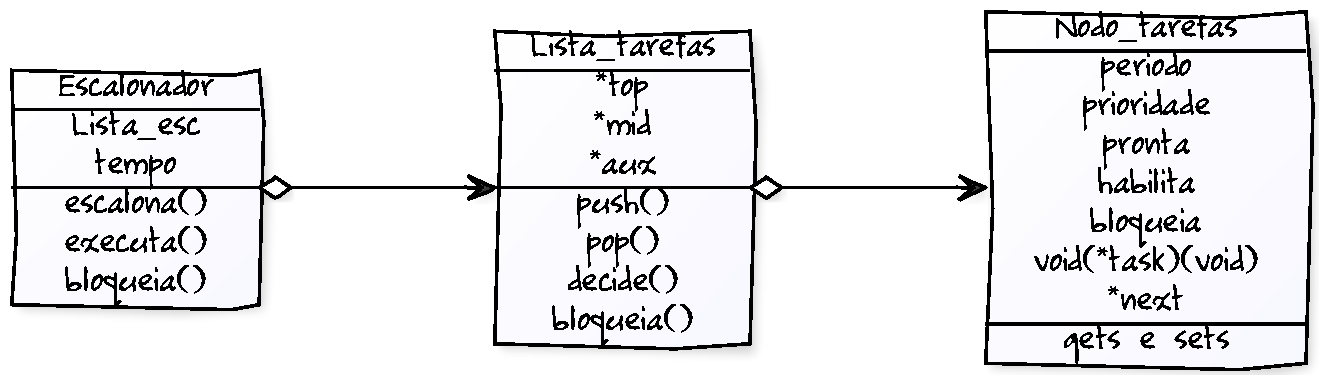
\includegraphics[width=0.85\textwidth]{diag_cla_esc.pdf}
        \caption{\small{Diagrama expandido das classes envolvidas no escalonamento.}}
        \label{fig:diag_cla_esc}
    \end{center}
\end{figure}

As tarefas que são inseridas nessa lista são às refentes à máquina de vendas, ao Banco de Dados, e às classes de manutenção do horário e calendário, conforme mostrado no código abaixo:


\begin{minted}
[
fontsize=\small,
linenos
]{cpp}
int main()
{
    Escalonador Escalonador;

    //periodo, prioridade, pronta, habilitada, bloqueada, funcao
                                 
    Escalonador.escalona(30, 1, 0, 1, 0, &sell);  

    Escalonador.escalona(50, 2, 0, 1, 0, &repor); 

    Escalonador.escalona(1000, 3, 0, 1, 0, &atualiza_tempo);

    while (true)
    {
        Escalonador.executa();
        usleep(1000); //1ms
    }
}
\end{minted}

O escalonamento do ClockCalendar, por exemplo, na linha 11, recebeu um período de 1000 ms pois deve ser chamado a cada 1 segundo para atualizar a hora. Este também recebeu a prioridade mais alta entre as tarefas para evitar erros cumulativos na manutenção do horáio. A função sell() chama a função venda() de machine, no entanto isso é feito através da criação de uma thread, pois no caso da interface com o microcomputador a função get\_entrada() da classe InterfacePC utiliza o comando cin, o qual é impossível interromper sem que o usuário pressione enter. Dessa forma, chamando como uma thread, não há um boqueio do escalonador por esperar o retorno desta função.


\large
\vspace{20pt}
 \textbf {6. Testes }
\vspace{10pt}
\normalsize

Como estratégia para os testes foram utilizados diversos mains locais, que possibilitaram testar extensivamente as os diversos módulos do projeto acarretando na correção de diversos casos de borda e comportamentos inesperados. Foram criados mains locais para as classes do banco de dados, do escalonador, da máquina de vendas e do calendário e do clock. 

No caso do Escalonador, por exemplo, foram criadas 4 funções de teste com períodos e prioridades distintas e passadas para a fila de tarefas através de um main local. Foi possível escalonar essas tarefas para 500 unidades de tempo e verificar o desempenho do algoritmo em casos de conflito de execução,  precedência de prioridades e assim por diante. O código deste main bem como seu resultado é apresentado no APÊNDICE 3. 

\large
\vspace{20pt}
 \textbf {7. Considerações finais }
\vspace{10pt}
\normalsize

A solução de escalonamento apresentada neste relatório não é preemptiva uma vez que não foi encontrada uma maneira de interromper e salvar contexto de uma tarefa em execução sem ter acesso aos registros de baixo nível. Para evitar que o escalonador fique preso majoritariamente na função de venda,  esperando input, foi usada estratégia de criação de uma thread para esta função. Para as demais funções não foi considerado necessária a criação de threads, já que suas execuções são relativamente rápidas. 

A estrutura modular e com possibilidade de reuso proporcionada pela orientação a objetos facilitou muito a organização e o desenvolvimento dos códigos. Foi possível implementar um código muito bem estruturado e "limpo", com detalhes das implementações ficando dentro das respectivas classes e funções. Com algumas modificações e adaptações foi possível reutilizar as classes de nodo e lista do banco de dados para o escalonador. Além disso, o uso de bibliotecas prontas para realizar tarefas específicas foi cruicial, como o uso da pthread para criação de threads. 

Algumas funções importantes não puderam ser usadas na plataforma Atlys, como a função usleep(), to\_string() e pthread\_create(). Alternativas foram implementadas para substitui-las como, por exemplo, um for para o delay. Os relatórios de compilação, tanto no Linux como na plataforma alvo, estão incluidos nos Apêndices 4 e 5. 

O projeto foi desafiador e possibilitou grande aprendizado ao longo do desenvolvimento, seja sobre as regras do C++, funcionamento de estruturas de dados ou mesmo sobre o paradigma de orientação a objeto. 

















\pagebreak
\large
\vspace{30pt}
 \textbf {APÊNDICE 1 - Manual do usuário}
\vspace{10pt}
\normalsize

Para compilar o código atual em um sistema Linux com o g++, basta definir PC (\#define PC) e digitar as linhas de comando abaixo: 
\begin{minted}
[
fontsize=\small,
linenos
]{cpp}
g++ -o exe main.cpp -pthread
./exe
\end{minted}

Para compilar o código atual no sistema embarcado alvo, basta definir ATL (\#define ATL) salvar e seguir os passos do tutorial de uso da Placa Atlys. Note que não há necessidade do uso da pthread neste caso.  

Com o programa em execução, para usar a máquina de refrigerantes basta inserir moedas seguindo o padrão "m" + valor. Por exemplo, para inserir uma moeda de R\$ 1,00 basta digitar "m100" e pressionar enter. Para moedas abaixo de  R\$ 1,00 deve-se inserir um "0" entre "m" e o valor, como em "m050". Para pedir um refrigerante do tipo MEET basta digitar "meet" e pressionar enter e, similarmente, "etirps" para um refrigerante do tipo Sprite. As devoluções de valores ocorrem no padrão "d" + valor, sendo que para solicitar uma devolução de valores basta digitar "dev". 

Para solicitar o relatório com o período de mais vendas, o refrigerante mais vendido e o valor de vendas, basta digitar "report" e pressionar enter. Há, ainda, a função de listar cada uma das vendas já realizadas desde que a máquina iniciou funcionamento, através do comando "report.all".


Para usar a classe Escalonador no seu projeto basta criar um objeto tipo Escalonador e e chamar a função escalona() com os atributos período, prioridade (quanto maior o número mais prioritária), flag de pronta, flag de habilitada, flag de bloqueada, e o endereço para a funão a ser escalonada (do tipo void (void)), respectivamente. Em seguida, para que haja execução é necessário chamar a função executa(). Sempre a que esta função for chamada haverá um incremento do tempo mantido pelo escalonador, portanto, se executa() for chamada a cada milissegundo o período das tarefas (passado como argumento da função escalona()) será dado em milissegundos. 

O código abaixo é um exemplo de como usar a classee Escalonador: 

\begin{minted}
[
fontsize=\small,
linenos
]{cpp}

#include "Escalonador.cpp"

int main()
{
    Escalonador Escalonador;

    Escalonador.escalona(int periodo, int prioridade, int pronta, int habilitada,
    int bloqueada, void()(void) funcao);

    while (true)
    {
        Escalonador.executa();
        usleep(1000); //1ms
    }
}
\end{minted}



\pagebreak
\large
\vspace{30pt}
 \textbf {APÊNDICE 2 - Algoritmo de decisão do escalonador}
\vspace{10pt}
\normalsize
\\
\begin{minted}
[
fontsize=\small,
linenos
]{cpp}
void ListaEsc::decide(unsigned long int tempo)
{
    void (*ttt)(void);
    int exec = 0;
    int ptr = 0;

    //periodo, prioridade, pronta, habilitada, bloqueada, funcao

    if (top) //se existe no na lista
    {
        //varre a fila para por na fila das prontas

        mid = top; //meio aponta para o topo da lista

        while (mid != 0) //enquanto meio nao chega no fim da lista
        {
            if (mid->get_habilita() && !mid->get_bloqueada()) // se
            //a tarefa esta habilitada
            {
                if ((tempo - mid->get_count()) == mid->get_periodo()) 
                // se seu periodo ja passou
                {
                    mid->set_count(tempo); // momento de 
                    //execucao = momento atual

                    ptr = mid->get_pronta(); // pega o valor de 
                    //quantas vezes a tarefa ficou pronta para 
                    //executar

                    ptr++; //incrementa esse valor

                    mid->set_pronta(ptr); // poe na fila das prontas

                    ptr = 0; // zera variavel auxiliar

                    if (mid->get_prioridade() > n) // se a prioridade
                    //dessa tarefa for maior que a prioridade teto
                    {
                        n = mid->get_prioridade(); // seta para ser 
                        //a prioridade teto
                    }
                }
            }

            mid = mid->get_next(); // meio aponta para o proximo
            //nodo
        }

        //varre a fila novamente para executar a de maior
        prioridade na fila das prontas

        while (exec == 0) // enquanto nao executar algo varre 
        //a fila e diminui a prioridade teto
        {
            mid = top; //meio aponta para o topo da lista

            while (mid != 0) //enquanto meio nao chega no fim da 
            //lista
            {
                if (mid->get_pronta() > 0 && !exec) // entra as
                prontas
                {
                    if (mid->get_prioridade() == n &&
                    !mid->get_bloqueada()) // acha a que tem 
                    //prioridade igual a prioridade mais alta 
                    /entre as prontas
                    {
                        ptr = mid->get_pronta(); //pega o valor de
                        pronta
                        ptr = ptr - 1;           // diminui
                        mid->set_pronta(ptr);    // seta
                        ptr = 0;                 //zera 
                        //variavel auxiliar

                        ttt = mid->get_void(); // pega endereco
                        //da funcao
                        ttt();                 // executa
                        exec = 1;              //houve uma execucao
                    }
                }

                mid = mid->get_next(); // meio aponta para o proximo
               // nodo
            }

            n = n - 1; // diminui a lista da maior prioridade

            if (n < 0) // caso a prioridade teto desceu a zero e 
           // nada foi executado
            {
                mid = top; //meio aponta para o topo da lista

                while (mid != 0) //enquanto meio nao chega no fim 
                //da lista
                {
                    if (mid->get_pronta() > 0 && !exec) // entra
                    //as prontas
                    {
                        ptr = mid->get_pronta(); //pega o valor 
                       // de pronta
                        ptr = ptr - 1;           // diminui
                        mid->set_pronta(ptr);    // seta
                        ptr = 0;                 //zera variavel
                        //auxiliar

                        ttt = mid->get_void(); // pega endereco 
                        //da funcao
                        ttt();                 // executa
                        exec = 1;              //houve uma execucao
                    }

                    mid = mid->get_next(); // meio aponta para 
                    //o proximo nodo
                }
                exec = 1;
            }
        }
    }
}


\end{minted}



\pagebreak
\large
\vspace{30pt}
 \textbf {APÊNDICE 3 - Main local para testes do escalonador}
\vspace{10pt}
\normalsize

\begin{minted}
[
fontsize=\small,
linenos
]{cpp}

#include <iostream>
#include <string>
#include <stdlib.h>
#include <unistd.h>

using namespace std;

#include "Escalonador.cpp"

void foo()
{
    cout << "     T2  P2";
}

void foo2()
{
    cout << "     T5  P4";
}

void foo3()
{
    cout << "     T10  P3";
}

void foo4()
{
    cout << "     T1  P1";
}

int main()
{
    Escalonador Escalonador;
    
   //periodo, prioridade, pronta, habilitada, bloqueada, funçao
    Escalonador.escalona(1, 1, 0, 1, 0, &foo4);
    Escalonador.escalona(2, 2, 0, 1, 0, &foo);
 
    Escalonador.escalona(5, 4, 0, 1, 0, &foo2);
    Escalonador.escalona(10, 3, 0, 1, 0, &foo3);

    int b = 0;

    while (b < 500)
    {
        Escalonador.executa();
        b++;

        if (b == 100)
            Escalonador.bloqueia(&foo4);

        usleep(1000); //1ms
    }
}


\end{minted}
Output:
\begin{minted}
[
fontsize=\small,
linenos
]{cpp}
t1      T1  P1
t2      T2  P2
t3      T1  P1
t4      T2  P2
t5      T5  P4
t6      T2  P2
t7      T1  P1
t8      T2  P2
t9      T1  P1
t10      T5  P4
t11      T10  P3
t12      T2  P2
t13      T1  P1
t14      T2  P2
t15      T5  P4
t16      T2  P2
t17      T1  P1
t18      T2  P2
t19      T1  P1
t20      T5  P4
...

\end{minted}



\pagebreak
\large
\vspace{30pt}
 \textbf {APÊNDICE 4 - Relatório de compilação no Linux}
\vspace{10pt}
\normalsize

\begin{minted}
[
fontsize=\small,
linenos
]{cpp}
ca_rigo@DESKTOP-0G0MJHJ:/mnt/d/OneDrive/_education/_doutorado/_materias/
_C++/_trabalho_final/vending_machine/vending_machine$ g++ -o exe main.cpp -pthread

In file included from Machine/../Dados/Pilha.cpp:2:0,
                 from Machine/../Dados/BancoDados.h:8,
                 from Machine/Machine.h:5,
                 from Machine/Machine.cpp:1,
                 from functions.cpp:6,
                 from main.cpp:5:
Machine/../Dados/../common.h:4:12: warning: ‘g_data’ initialized and declared 
‘extern’
 extern int g_data = 0;
            ^~~~~~
Machine/../Dados/../common.h:5:12: warning: ‘g_hora’ initialized and declared 
‘extern’
 extern int g_hora = 0;
            ^~~~~~
Machine/../Dados/../common.h:6:12: warning: ‘repo’ initialized and declared ‘extern’
 extern int repo = 0;
            ^~~~
Machine/../Dados/../common.h:7:12: warning: ‘repo1’ initialized and declared ‘extern’
 extern int repo1 = 0;
            ^~~~~
Machine/../Dados/../common.h:8:12: warning: ‘th’ initialized and declared ‘extern’
 extern int th = 0;




\end{minted}



\pagebreak
\large
\vspace{30pt}
 \textbf {APÊNDICE 5 - Relatório de compilação na plataforma Atlys}
\vspace{10pt}
\normalsize

\begin{minted}
[
fontsize=\small,
linenos
]{cpp}
alunos@LABSDG-03:~/Desktop/vending_machine$ sparc-elf-g++ main.cpp -o programa

In file included from Machine/../Dados/Pilha.cpp:2,
                 from Machine/../Dados/BancoDados.h:8,
                 from Machine/Machine.h:5,
                 from Machine/Machine.cpp:1,
                 from functions.cpp:6,
                 from main.cpp:5:
Machine/../Dados/../common.h:4: warning: 'g_data' initialized and declared 'extern'
Machine/../Dados/../common.h:5: warning: 'g_hora' initialized and declared 'extern'
Machine/../Dados/../common.h:6: warning: 'repo' initialized and declared 'extern'
Machine/../Dados/../common.h:7: warning: 'repo1' initialized and declared 'extern'
Machine/../Dados/../common.h:8: warning: 'th' initialized and declared 'extern'
alunos@LABSDG-03:~/Desktop/vending_machine$ 





\end{minted}






\end{document}